% !TEX root = cikm2018-visual-ltr.tex

\section{Dataset}\label{sec:dataset}
In this section, we describe the \datasetname~data\-set. Section~\ref{sec:trecclue} contains information about the underlying ClueWeb12 collection and TREC Web Track topics. Section~\ref{sec:screenshotsec} explains how the snapshots for ClueWeb12 were acquired using the Wayback Machine\footnote{\url{TODO}} and ClueWeb12 Online rendering service.\footnote{\url{TODO}} Section~\ref{sec:contentfeature} discusses the details on how content features, such as BM25 and TF-IDF, are calculated using Apache Spark.\footnote{\url{TODO}} Finally, Section~\ref{sec:finalcollection} gives an overview of the structure in which the \datasetname dataset is presented.

\subsection{ClueWeb12 \& TREC Web Track}\label{sec:trecclue}
ClueWeb12 is a highly diverse collection of web pages scraped in the first half of 2012.
The total collection contains over 700 million documents that are crawled using the typical crawling settings of the Heritrix archival crawler project.\footnote{\url{https://webarchive.jira.com/wiki/spaces/Heritrix/overview}}
\todo{We build on this collection/we picked this collection, because \ldots}
\todo{We use only judged documents discussed next!}

\datasetname~uses the topics from the TREC Web Tracks 2013 \& 2014~\cite{collins2013trec,collins2015trec} as queries.
\todo{Again, why do we use these query sets?}
Table~\ref{tab:countsources} shows a breakdown of the total number of documents, queries and different relevance labels of the combined sets of 2013 and 2014.
\todo{Is there anything special about this table and numbers that we can mention here?}

\begin{table}[h]
  \captionof{table}{A breakdown of the relevance judgments for the TREC Web Track and the amount of snapshots taken from the Wayback machine and ClueWeb12 rendering service.} 
  \label{tab:countsources}
  \begin{tabular}{ l | r | r  r  r }
  \toprule
    Count/Label & TREC Web & Wayback & ClueWeb12 & No image\\
    \midrule
    Total & 28,906 & 23,249 & 5,392 & 265 \\
    Nav grade (4) & 40 & 36 & 4 & 0\\
    Key grade (3) & 409 & 347 & 62 & 0\\
    Hrel grade (2) & 2,534 & 2,222 & 295 & 17 \\
    Rel grade (1) & 6,832 & 5,679 & 1,123 & 30\\
    Non grade (0) & 18,301 & 14,395 & 3,701 & 205 \\
    Junk grade (-2) & 790 & 570 & 207 & 13\\
    \bottomrule
  \end{tabular} 
\end{table}


\subsection{Snapshots} \label{sec:screenshotsec}
%
%\begin{table*}[t]
%\begin{center}
%\begin{tabular}{llllllll}
%\multicolumn{8}{c}{Clueweb12 11 features}                                    \\ 
%                      & P@1   & P@5   & P@10  & NDCG@1 & NDCG@5 & NDCG@10 & MAP   \\ \hline
%BM25                  & 0.300 & 0.319 & 0.316 & 0.153  & 0.197  & 0.188   & 0.350 \\ \hline
%RankBoost             & 0.420 & 0.432 & 0.441 & 0.244  & 0.270  & 0.285   & 0.423 \\
%AdaRank               & 0.260 & 0.362 & 0.377 & 0.132  & 0.203  & 0.228   & 0.383 \\
%LambdaMart            & 0.440 & 0.442 & 0.467 & 0.243  & 0.268  & 0.294   & 0.434 \\ \hline
%ViP baseline          & 0.338 & 0.359 & 0.370 & 0.189  & 0.215  & 0.233   & 0.415 \\ \hline
%%ViP masks             & 0.346 & 0.391 & 0.399 & 0.186  & 0.232  & 0.251   & 0.419 \\
%ViP highlights        & 0.418 & 0.409 & 0.416 & 0.239  & 0.253  & 0.269   & 0.422 \\
%ViP snapshots         & 0.392 & 0.389 & 0.398 & 0.217  & 0.238  & 0.254   & 0.421 \\ \hline
%VGG snapshots      & 0.514 & 0.488 & 0.484 & 0.292  & 0.307  & 0.324   & 0.442 \\ 
%VGG highlights     & 0.560 & 0.547 & 0.520 & 0.323  & 0.337  & 0.346   & 0.456 \\ \hline
%VGG saliency       & 0.554 & 0.478 & 0.453 & 0.310  & 0.296  & 0.302   & 0.422 \\
%\end{tabular}
%\centering
%\captionof{table}{Results after 5 iterations on all 5 folds of \datasetname. ViP is the model by \citet{fan2017learning}, the baseline uses only content features and VGG-16 is the pre-trained feature extractor.}
%\label{tab:results}
%\end{center}
%\end{table*}

%\begin{table*}[h]
%\caption{A benchmark comparison between the MQ2007 query set using all 46 LETOR features and the 11 LETOR features that are used in \datasetname.}
%\label{tab:11vs46}
%\centering
%\begin{tabular}{lccccccc}
%\toprule
%%& \multicolumn{7}{c}{MQ2007 46 features vs 11 features}                                     \\
%           & P@1    & P@5    & P@10   & NDCG@1 & NDCG@5 & NDCG@10 & MAP    \\ 
%\midrule
%RankBoost - 46  & 0.453 & 0.404 & 0.371 & 0.391 & 0.403 & 0.430  & 0.457 \\
%RankBoost - 11 & 0.448 & 0.400 & 0.372 & 0.381  & 0.401  & 0.431   & 0.453 \\
%\midrule
%AdaRank - 46  & 0.420 & 0.402 & 0.360 & 0.367 & 0.403 & 0.424  & 0.449 \\
%AdaRank - 11  & 0.385 & 0.391 & 0.287 & 0.364  & 0.396  & 0.394   & 0.386 \\ 
%\midrule
%LambdaMart - 46 & 0.452 & 0.418 & 0.384 & 0.405 & 0.411 & 0.444  & 0.463 \\
%LambdaMart - 11 & 0.448 & 0.412 & 0.380 & 0.397  & 0.411  & 0.443   & 0.455 \\
%\bottomrule
%\end{tabular}
%\end{table*}


\subsubsection{Acquisition}
Although each entry in the ClueWeb12 collection contains the document's HTML source, many pages lack the required styling and images files in order to render the full page. Instead, the pages are rendered using the Wayback Machine\footnote{\url{http://archive.org/web/}} from Archive.org which offers various archived versions of web pages with styling and images since 2005. Scraping was performed on the available entry on the Wayback Machine that is closest to the original scrape date. A snapshot is then taken using a headless instance of the Firefox browser together with the Python implementation of the Selenium\footnote{\url{http://selenium-python.readthedocs.io/}} testing framework. 
For reproduction of the work from \citet{fan2017learning}, we created a separate query dependent dataset with the same snapshots where all query words are highlighted in red (HEX value: \#ff0000).

\begin{figure}[h]
\begin{tabular}{ccc}
\subfloat{
\includegraphics[width = 1in]{images/1-snapshot.png}} &
\subfloat{
\includegraphics[width = 1in]{images/1-highlights.png}} &
\subfloat{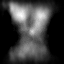
\includegraphics[width = 1in]{images/1-saliency.png}} \\
\subfloat{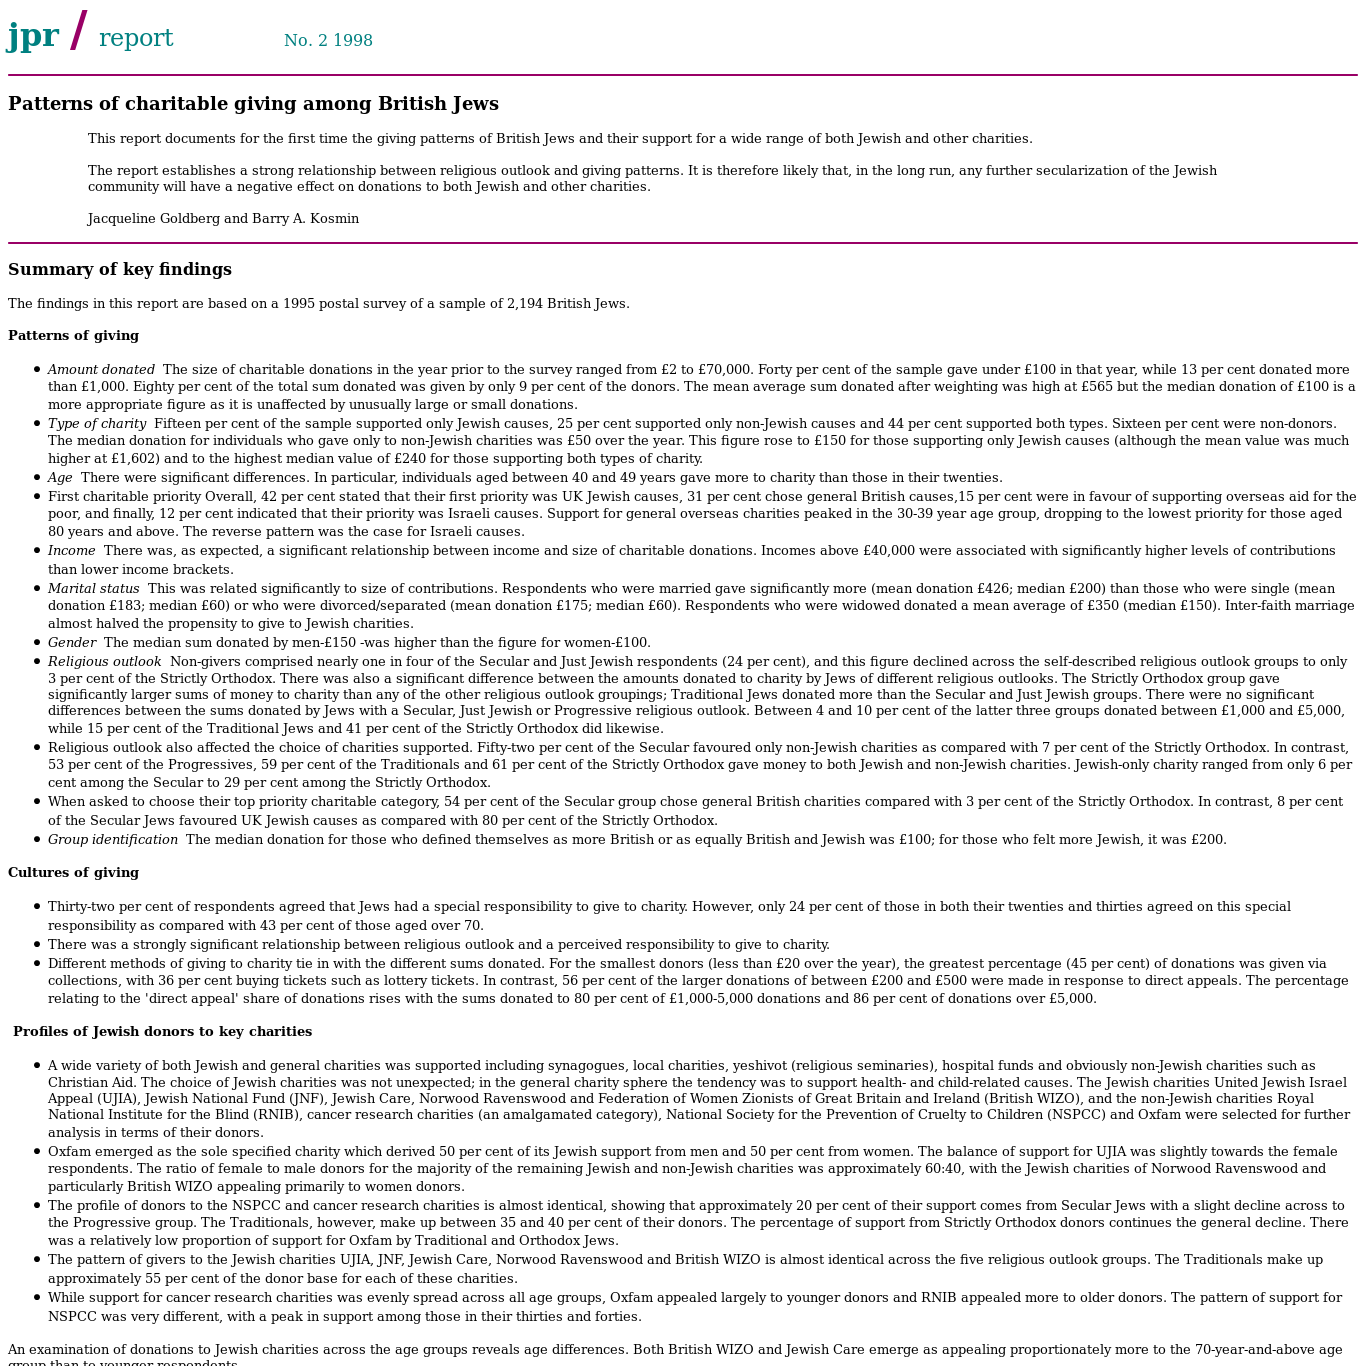
\includegraphics[width = 1in]{images/2-snapshot.png}} &
\subfloat{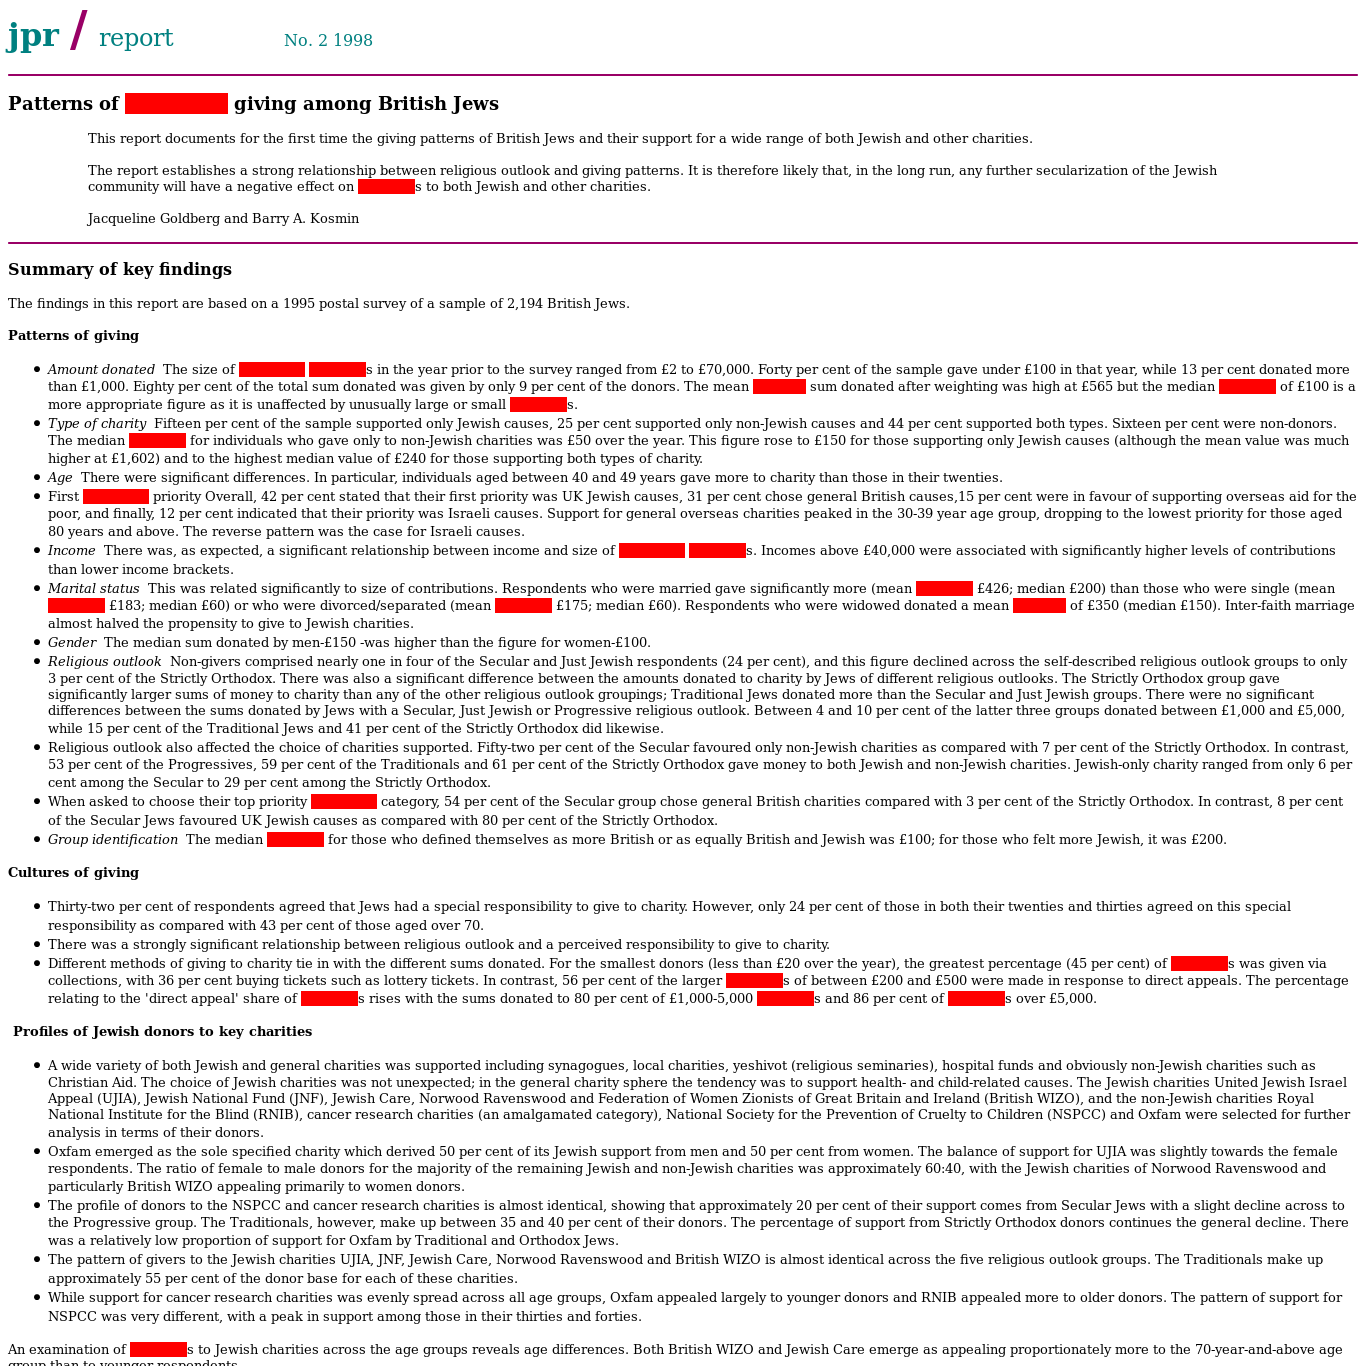
\includegraphics[width = 1in]{images/2-highlights.png}} &
\subfloat{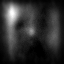
\includegraphics[width = 1in]{images/2-saliency.png}} \\
\subfloat{
\includegraphics[width = 1in]{images/3-snapshot.png}} &
\subfloat{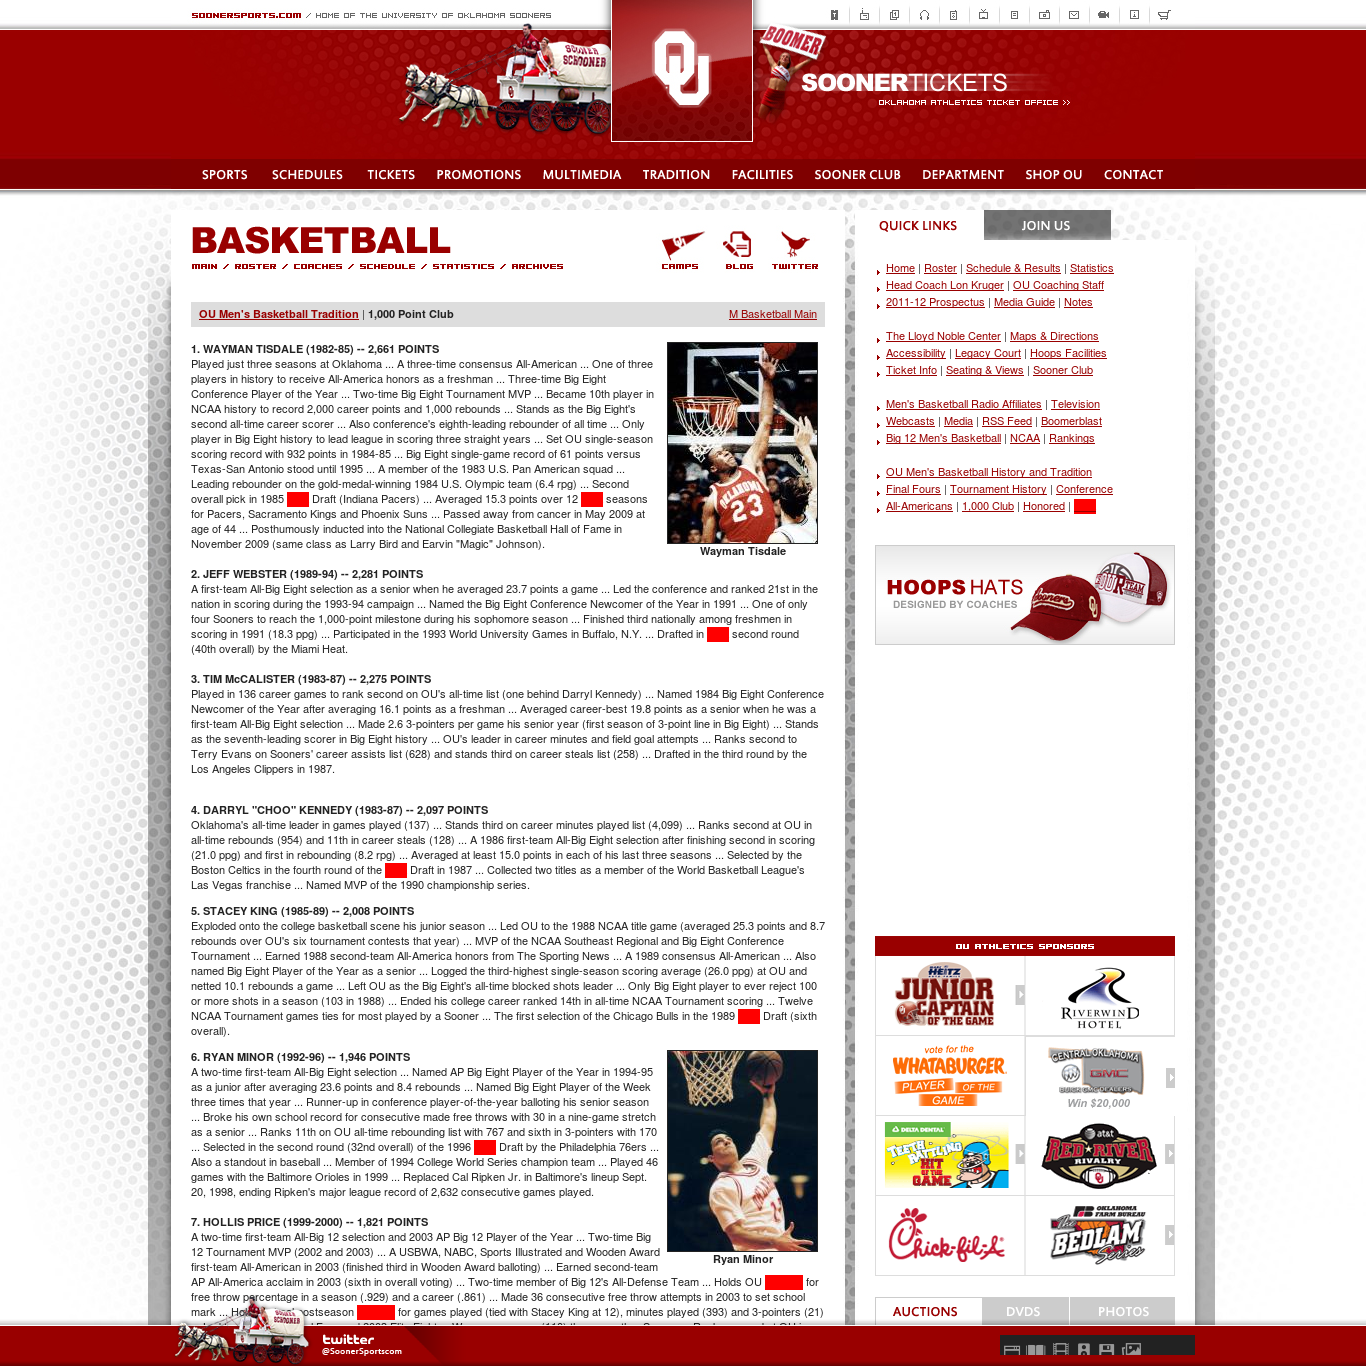
\includegraphics[width = 1in]{images/3-highlights.png}} &
\subfloat{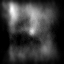
\includegraphics[width = 1in]{images/3-saliency.png}} \\
\end{tabular}
\caption{Examples of the vanilla snapshot, red highlighted snapshot and saliency heatmap from left to right respectively}\label{fig:exampleshots}
\end{figure}

\subsubsection{Filtering}\label{sec:datasetsum}
As the Wayback Machine does not contain an archived or working version of each document in the ClueWeb12 collection, a filtering process was introduced to maximize the quality of each snapshot. Using the following criteria, a snapshot was selected for each available document. 
\begin{enumerate}    
\item Each document was requested from the Wayback Machine separately. 
\item Documents that were not on the Wayback Machine, timed out, threw a JavaScript error or resulted in a .PNG snapshot smaller than 100kb are marked as broken. These documents are rendered again with the ClueWeb12 html using the online rendering service provided by the creators of ClueWeb12.
\item A manual selection was made between all documents that were rendered from both sources: The Wayback version was used if it contained more styling elements and if the content was the same as the rendering service. Otherwise, the rendering service version was used. 
\item In total, 265 documents were discarded because of issues during rendering.
\end{enumerate}

At the end of the process, each a total of 28,906 judged documents have a corresponding snapshot from either the Wayback Machine or ClueWeb12 rendering service. Table \ref{tab:countsources} shows how the different sources are divided.


\subsection{Content features} \label{sec:contentfeature}
In LTR, documents are ranked based on various calculated content features. We computed these content features by doing a full pass over the complete ClueWeb12 using Apache Spark. This took approximately 20 hours on 116 Hadoop worker nodes with 3 executor cores and 21gb memory each. During this process an HTML parser (\textit{jsoup}\footnote{{\url{https://jsoup.org/}}}) extracted the title and content from the raw HTML. Because the HTML structure in some larger documents could not be parsed efficiently by jsoup, all documents with more than one million tokens were ignored. Using the Apache Spark 2.2.1 implementation of TF and IDF, a sparse vector was obtained for each item in each document.  On top of the IR features, PageRank scores from the ClueWeb12 \textit{Related Data} section\footnote{{\url{https://lemurproject.org/clueweb12/related-data.php}}} were added to each document as well. In total, 11 features are computed of which a full overview can be found in Table \ref{tab:setdescription}. Finally, the following modifications based on the features from LETOR 3.0 \cite{qin2010letor} were made to stabilize training:
\begin{enumerate}  
% \item IDF is calculates as follows: 
% $$IDF(q, D) = \sum_{t_i \in q} IDF(t_i, D) = \sum_{t_i \in t} \log \frac{|D| + 1}{DF(t_i) + 1}$$
% Where  $q_i$ and $t_i$ represent a list of all terms in a query and a single query term respectively. $D$ represents a list of all terms in a document with $|D|$ as its total length. $DF(t_i)$ is the document frequency for the given query term.  
\item Free parameters $k_1$, $k_3$ and $b$ for BM25 were set to $2.5$, $0$ and $0.8$ respectively. 
\item Because the PageRank score are usually an order of magnitude smaller than all the other scores, we multiplied each value with $10^5$.
\item After all features have been computed, the log is taken over the final results.
\item The logged features are normalized per query.  
\end{enumerate}

\begin{table}[h]
\centering
\captionof{table}{A description of all content features provided with \datasetname.}  \label{tab:setdescription} 
\begin{tabular}{lllrllrl}
\toprule
Id & Description &\qquad & Id & Description &\qquad & Id & Description    \\ 
\midrule
1  & Pagerank  && 5  & Content TFIDF  && 9  & Title IDF   \\
2  & Content length && 6  & Content BM25   && 10 & Title TFIDF   \\
3  & Content TF  && 7  & Title length && 11 & Title BM25  \\
4  & Content IDF && 8  & Title TF  && & \\
\bottomrule
\end{tabular}
\end{table}



%\textit{(This has not been done yet)} The TF and IDF scores were also calculated Anchor text extracted by \citet{hiemstra2010mapreduce} 
% Make a seperate section for snapshots and subsections for collection, cleaning, statistics etc.


\subsection{Final collection}\label{sec:finalcollection}
The process mentioned in the previous sections resulted in: 
\begin{inparaenum}[(i)]
\item a set of files containing the content features, and
\item a directory with snapshots.
\end{inparaenum}
The content features are stored in LETOR formatted files containing the raw, logged and query normalized values. The query normalized values were randomly split per query into five equal fold-partitions. There fold-partitions were then divided in five folds containing three fold-partitions for training and the remaining two for validation and testing. Each snapshot is stored as a .PNG which can be identified by its corresponding ClueWeb12 document id. 
%A separate file contains an entry for each snapshot indicating whether the snapshots was created using the Wayback Machine or online rendering service. 

%\begin{figure*}[t]
%\centering
%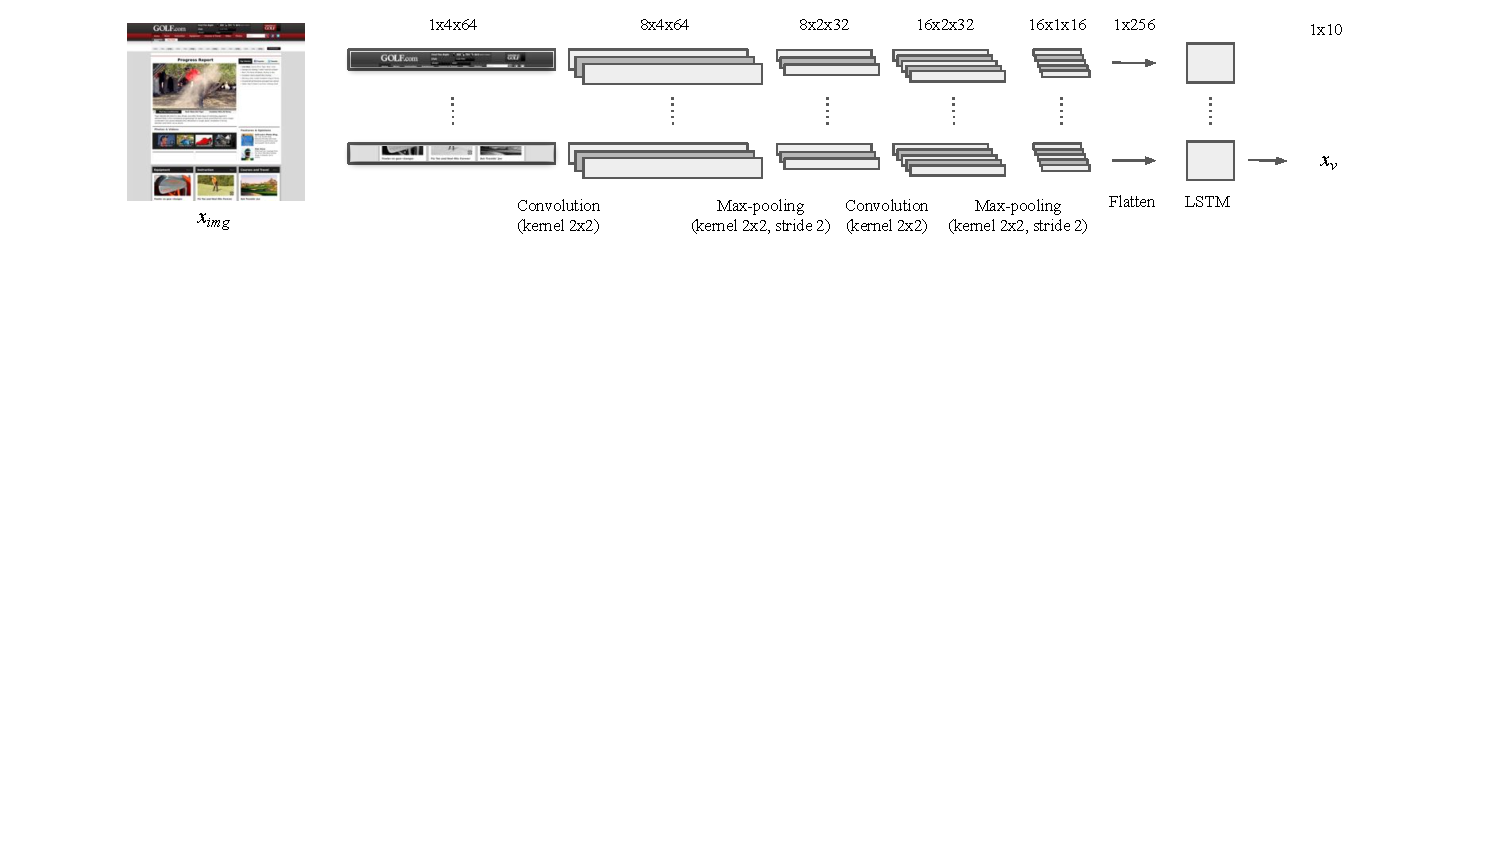
\includegraphics[clip,trim=0 10cm 0 0, width=20cm]{images/vip-features.pdf}
%  \captionof{figure}{The feature extractor architecture with corresponding dimensions used in our implementation of the ViP model.} \label{fig:ViPfeat} 
%\end{figure*}
